\documentclass[10pt]{article}
\usepackage[margin=1in]{geometry}
\usepackage{amsmath,amssymb,bm}
\usepackage{graphicx}
\usepackage{booktabs}
\usepackage{microtype}
\usepackage[hidelinks]{hyperref}
\usepackage[numbers,sort&compress]{natbib}
\usepackage{titlesec}
\usepackage{enumitem}
\linespread{0.94}
\setlist{nosep,leftmargin=*}
\titlespacing*{\section}{0pt}{0.75ex plus 0.2ex}{0.35ex}
\titlespacing*{\subsection}{0pt}{0.55ex plus 0.1ex}{0.25ex}
\titleformat{\section}{\normalsize\bfseries}{\thesection.}{0.4em}{}
\titleformat{\subsection}{\normalsize\bfseries}{\thesubsection.}{0.4em}{}
\setlength{\parindent}{0pt}
\setlength{\parskip}{2pt}
\setlength{\abovedisplayskip}{4pt}
\setlength{\belowdisplayskip}{4pt}
\setlength{\textfloatsep}{7pt}
\setlength{\floatsep}{6pt}
\setlength{\intextsep}{6pt}
\graphicspath{{../../experiments/sparc_nfw_residuals/figures/}}

\newcommand{\dd}{\mathrm{d}}
\newcommand{\cG}{\frac{8\pi G}{c^4}}
\newcommand{\Gobs}{G_{\mu\nu}[g^{\rm obs}]}
\newcommand{\Gbar}{G_{\mu\nu}[g^{\rm bar}]}
\newcommand{\Tmiss}{T^{\rm miss}_{\mu\nu}}

\title{Residual-of-Residual Geometry of NFW Fits to SPARC Rotation Curves}
\author{J. R. Landers}
\date{\vspace{-0.6em}May 2026}

\begin{document}
\maketitle
\vspace{-1.8em}

\begin{abstract}
This note applies a residual-of-residual diagnostic to public SPARC galaxy
rotation curves. The diagnostic follows the geometric-residual framework of
\citet{Landers2026a} and the synthetic NFW proof-of-concept in
\citet{Landers2026b}. For each usable SPARC galaxy, the baryon-subtracted
acceleration residual is computed from the observed rotation curve and fixed
stellar mass-to-light ratios, then fit with a pure Navarro-Frenk-White (NFW)
halo and a cored/isothermal control profile. The object of interest is not only
the fit score, but the leftover field
$\epsilon_g(R)=\Delta g_{\rm obs}(R)-\Delta g_{\rm candidate}(R)$.
Across 165 fitted galaxies, cored/isothermal residuals beat full-range NFW
fits in 78.8 percent of cases. In a primary-quality sample of 131 galaxies, the
fraction is 80.2 percent, and outer-region NFW fits leave a structured negative
inner residual in 51.9 percent of cases. The result is not a falsification of
cold dark matter. It is evidence that residual-of-residual fields are
measurable on real data and can classify where simple source geometries fail.
\end{abstract}

\section{Context}

The parent geometric-residual paper \citep{Landers2026a} recasts the
missing-mass problem as a comparison between the geometry inferred from
observations and the geometry predicted from baryons alone:
\begin{equation}
\Delta G_{\mu\nu}
:=
\Gobs-\Gbar,
\qquad
\Tmiss
:=
\frac{c^4}{8\pi G}\Delta G_{\mu\nu}.
\end{equation}
If ordinary general relativity is retained, a dark-matter model is a candidate
stress-energy source for this residual:
\begin{equation}
\Delta G_{\mu\nu}
\stackrel{?}{=}
\cG T_{\mu\nu}^{\rm candidate}.
\end{equation}

In weak-field disk galaxies, rotation curves mainly constrain the Newtonian
potential $\Phi$:
\begin{equation}
v^2(R)=R\frac{\dd\Phi}{\dd R}.
\end{equation}
The practical residual is therefore
\begin{equation}
\boxed{
\Delta g(R)
=
\frac{V_{\rm obs}^2(R)-V_{\rm bar}^2(R)}{R}.
}
\end{equation}
The synthetic NFW note \citep{Landers2026b} showed that a pure NFW profile can
match an outer flat-curve residual, but then tends to overpredict the central
residual in a controlled toy target. This paper asks whether the same
diagnostic can be applied to real astrophysical data.

\section{Data and Residual Construction}

The data are the public SPARC mass models of \citet{Lelli2016}, consisting of
175 disk galaxies with Spitzer photometry and accurate rotation curves. The
mass-model table gives, at each radius, $V_{\rm obs}$, its random uncertainty,
and the gas, disk, and bulge velocity contributions. The sample metadata
provide galaxy quality flags, inclinations, disk scale lengths, and flat-speed
estimates.

The baryonic contribution is computed using fixed fiducial stellar
mass-to-light ratios:
\begin{equation}
\Upsilon_{\rm disk}=0.5,
\qquad
\Upsilon_{\rm bulge}=0.7.
\end{equation}
Since the SPARC gas velocity contribution may be signed, the baryonic speed
term is
\begin{equation}
V_{\rm bar}^2
=
{\rm sign}(V_{\rm gas})V_{\rm gas}^2
+
\Upsilon_{\rm disk}V_{\rm disk}^2
+
\Upsilon_{\rm bulge}V_{\rm bul}^2.
\end{equation}
The observed residual acceleration is then
\begin{equation}
\Delta g_{\rm obs}(R)
=
\frac{V_{\rm obs}^2(R)-V_{\rm bar}^2(R)}{R}.
\end{equation}
The propagated acceleration uncertainty is approximated as
\begin{equation}
\sigma_{\Delta g}^2
=
\left[
\frac{2|V_{\rm obs}|\sigma_V}{R}
\right]^2
+
\left[
0.05\frac{V_{\rm obs}^2}{R}
\right]^2,
\end{equation}
where the second term is a modest systematic floor. This is not a full SPARC
halo-inference likelihood; it is a controlled residual-space diagnostic.

\section{Candidate Residual Families}

The NFW density profile \citep{Navarro1996} is
\begin{equation}
\rho_{\rm NFW}(r)
=
\frac{\rho_s}{(r/r_s)(1+r/r_s)^2}.
\end{equation}
With $x=r/r_s$,
\begin{equation}
M_{\rm NFW}(<r)
=
4\pi\rho_s r_s^3
\left[
\ln(1+x)-\frac{x}{1+x}
\right],
\end{equation}
so the residual acceleration is
\begin{equation}
\Delta g_{\rm NFW}(R)
=
\frac{G M_{\rm NFW}(<R)}{R^2}.
\end{equation}

The cored/isothermal control profile is
\begin{equation}
\Delta g_{\rm iso}(R)
=
\frac{v_0^2 R}{R^2+r_c^2}.
\end{equation}
It is included because it naturally approaches the flat-curve residual shape
$\Delta g\propto 1/R$ outside its core. A logarithmic-tail comparison
$\Delta g_{\log}=A/(R+R_0)$ is also fit, but the main physical comparison here
is NFW versus the cored/isothermal control.

The diagnostic field is
\begin{equation}
\boxed{
\epsilon_g(R)
=
\Delta g_{\rm obs}(R)
-
\Delta g_{\rm candidate}(R).
}
\end{equation}
For the outer-NFW test, NFW is fit only outside a galaxy-specific break radius,
chosen from $2.2R_{\rm disk}$ when available and clipped to the central
percentile range of the sampled radii. The question is then whether the NFW
halo required by the outer residual overpredicts the inner residual.

A spherical effective-density proxy is also computed for diagnostics:
\begin{equation}
\epsilon_\rho(R)
=
\frac{1}{4\pi G R^2}
\frac{\dd}{\dd R}
\left[
R^2\epsilon_g(R)
\right].
\end{equation}
This is not a disk mass inversion. It is a standardized way to compare the
sign and concentration of leftover source structure.

\section{Sample and Outputs}

The pipeline parsed 3,391 rotation-curve points for all 175 SPARC galaxies. Of
these, 165 galaxies had enough valid points for the fitting pipeline. The
primary-quality sample contains galaxies with SPARC quality flag 1 or 2, at
least 8 rotation-curve points, and inclination above 30 degrees when available.
This gives 131 galaxies. A stricter primary-flat subset requires measured
$V_{\rm flat}>0$, leaving 113 galaxies.

The experiment writes one row per galaxy, pointwise residual profiles, a
population summary, source metadata, and figures. All files are generated by
\texttt{run\_sparc\_nfw\_residuals.py}.

\begin{table}[t]
\centering
\small
\begin{tabular}{lrrrrrr}
\toprule
Sample & Galaxies & NFW RMSE & Cored RMSE & Cored beats NFW & Inner overshoot & Inner gap \\
\midrule
All fitted & 165 & 0.337 & 0.203 & 0.788 & 0.521 & -0.449 \\
Primary quality & 131 & 0.334 & 0.206 & 0.802 & 0.519 & -0.469 \\
Primary flat & 113 & 0.334 & 0.211 & 0.805 & 0.504 & -0.449 \\
\bottomrule
\end{tabular}
\caption{Population summary. NFW RMSE and cored RMSE are median full-range
relative RMSE values. ``Cored beats NFW'' is the fraction of galaxies where the
cored/isothermal weighted MSE is lower than the NFW weighted MSE. ``Inner
overshoot'' is the fraction where the outer-NFW fit leaves a structured
negative inner residual. ``Inner gap'' is the median normalized inner
$\epsilon_g$ after outer-NFW fitting.}
\label{tab:population}
\end{table}

\begin{figure}[t]
\centering
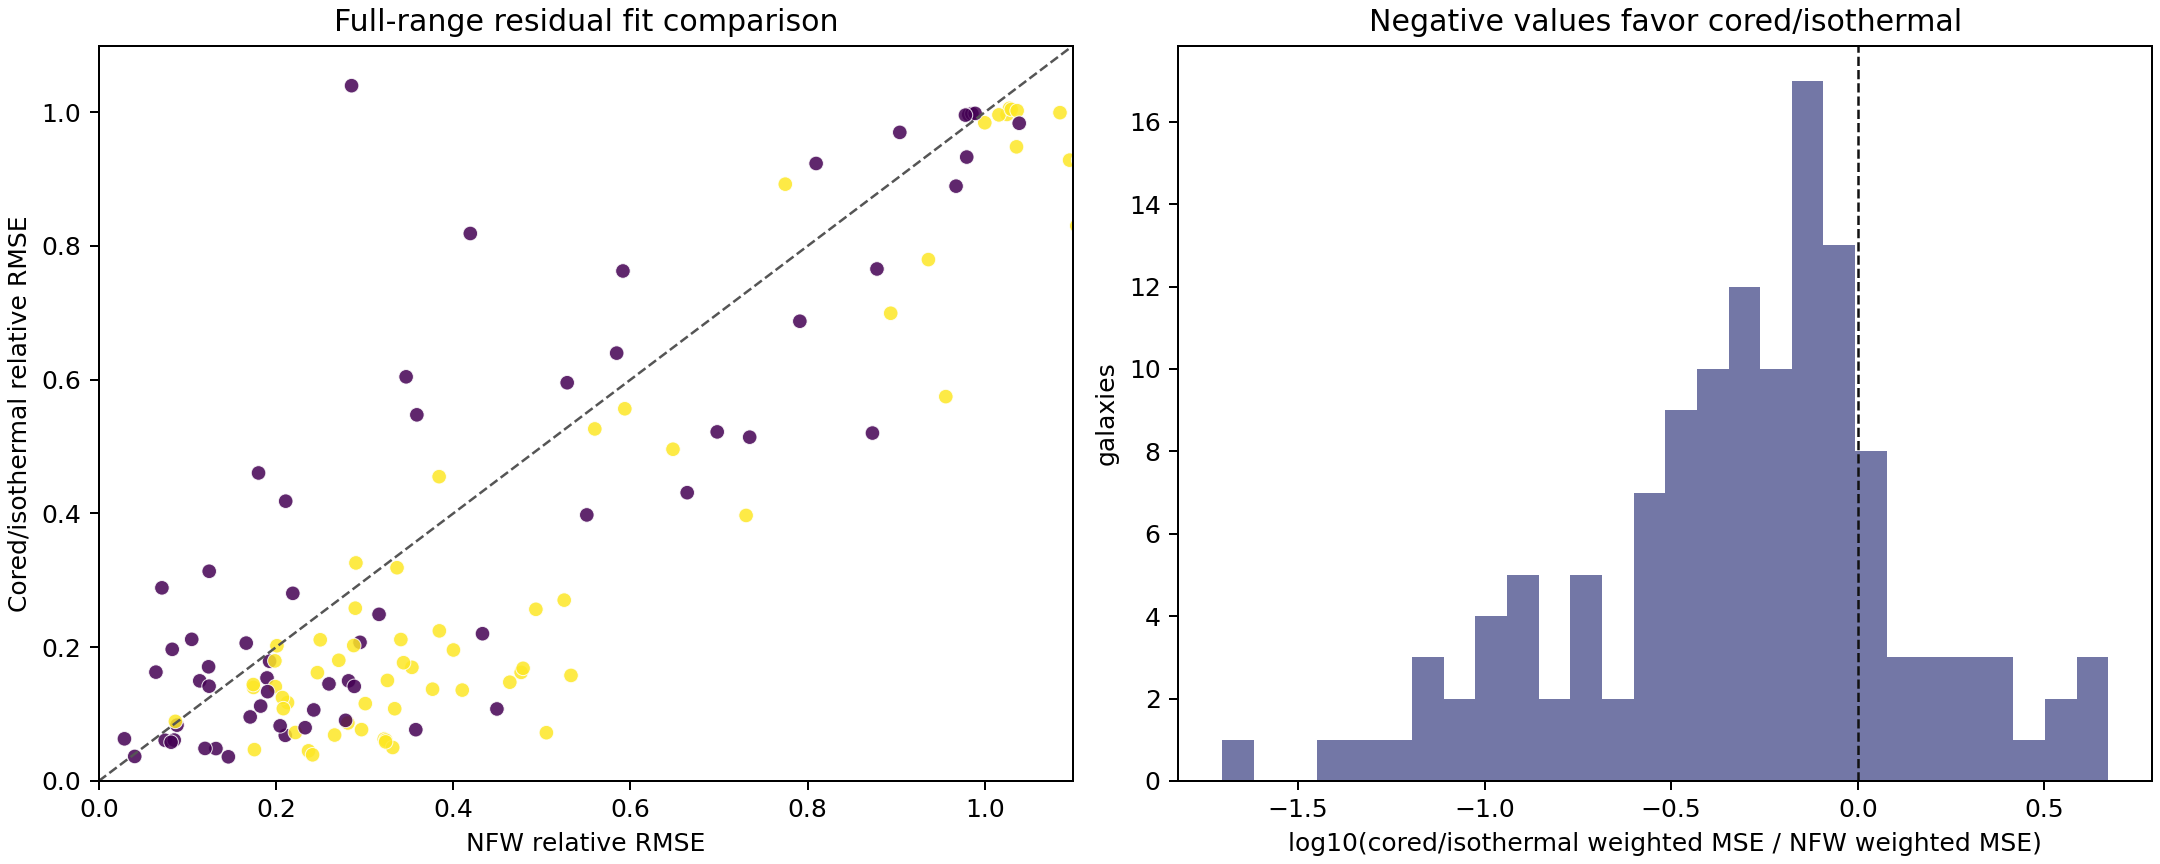
\includegraphics[width=\linewidth]{population_fit_comparison.png}
\caption{Population comparison of full-range residual fits. Left: each point
compares the NFW and cored/isothermal relative RMSE for one galaxy in the
primary-quality sample. Points below the dashed line favor the cored control.
Right: the distribution of weighted-MSE ratios is shifted negative, meaning
that cored/isothermal residuals beat NFW for most of the sample.}
\label{fig:population}
\end{figure}

\begin{figure}[t]
\centering
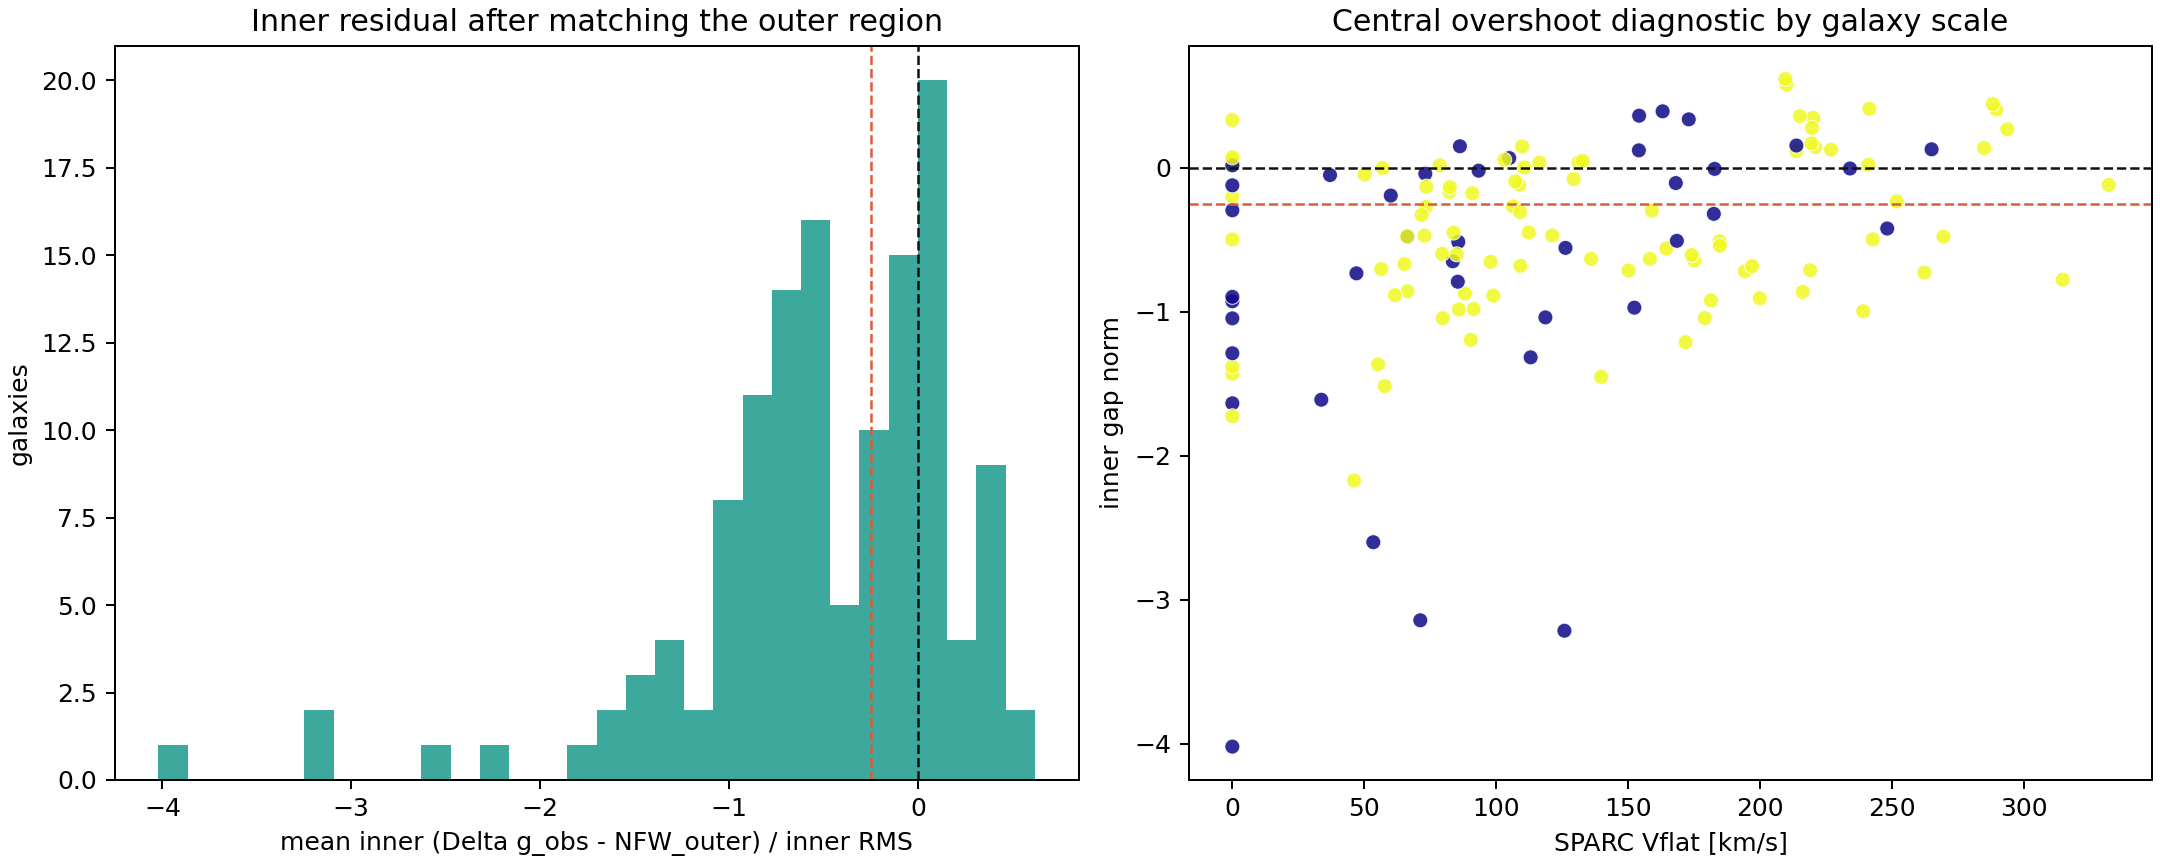
\includegraphics[width=\linewidth]{central_overshoot_distribution.png}
\caption{Residual-of-residual behavior after matching NFW to the outer region.
The left panel shows the distribution of normalized inner
$\Delta g_{\rm obs}-\Delta g_{\rm NFW,outer}$. The median is negative in every
reported sample. The right panel shows the same diagnostic against SPARC
$V_{\rm flat}$, with point color indicating the SPARC quality flag.}
\label{fig:overshoot}
\end{figure}

\begin{figure}[t]
\centering
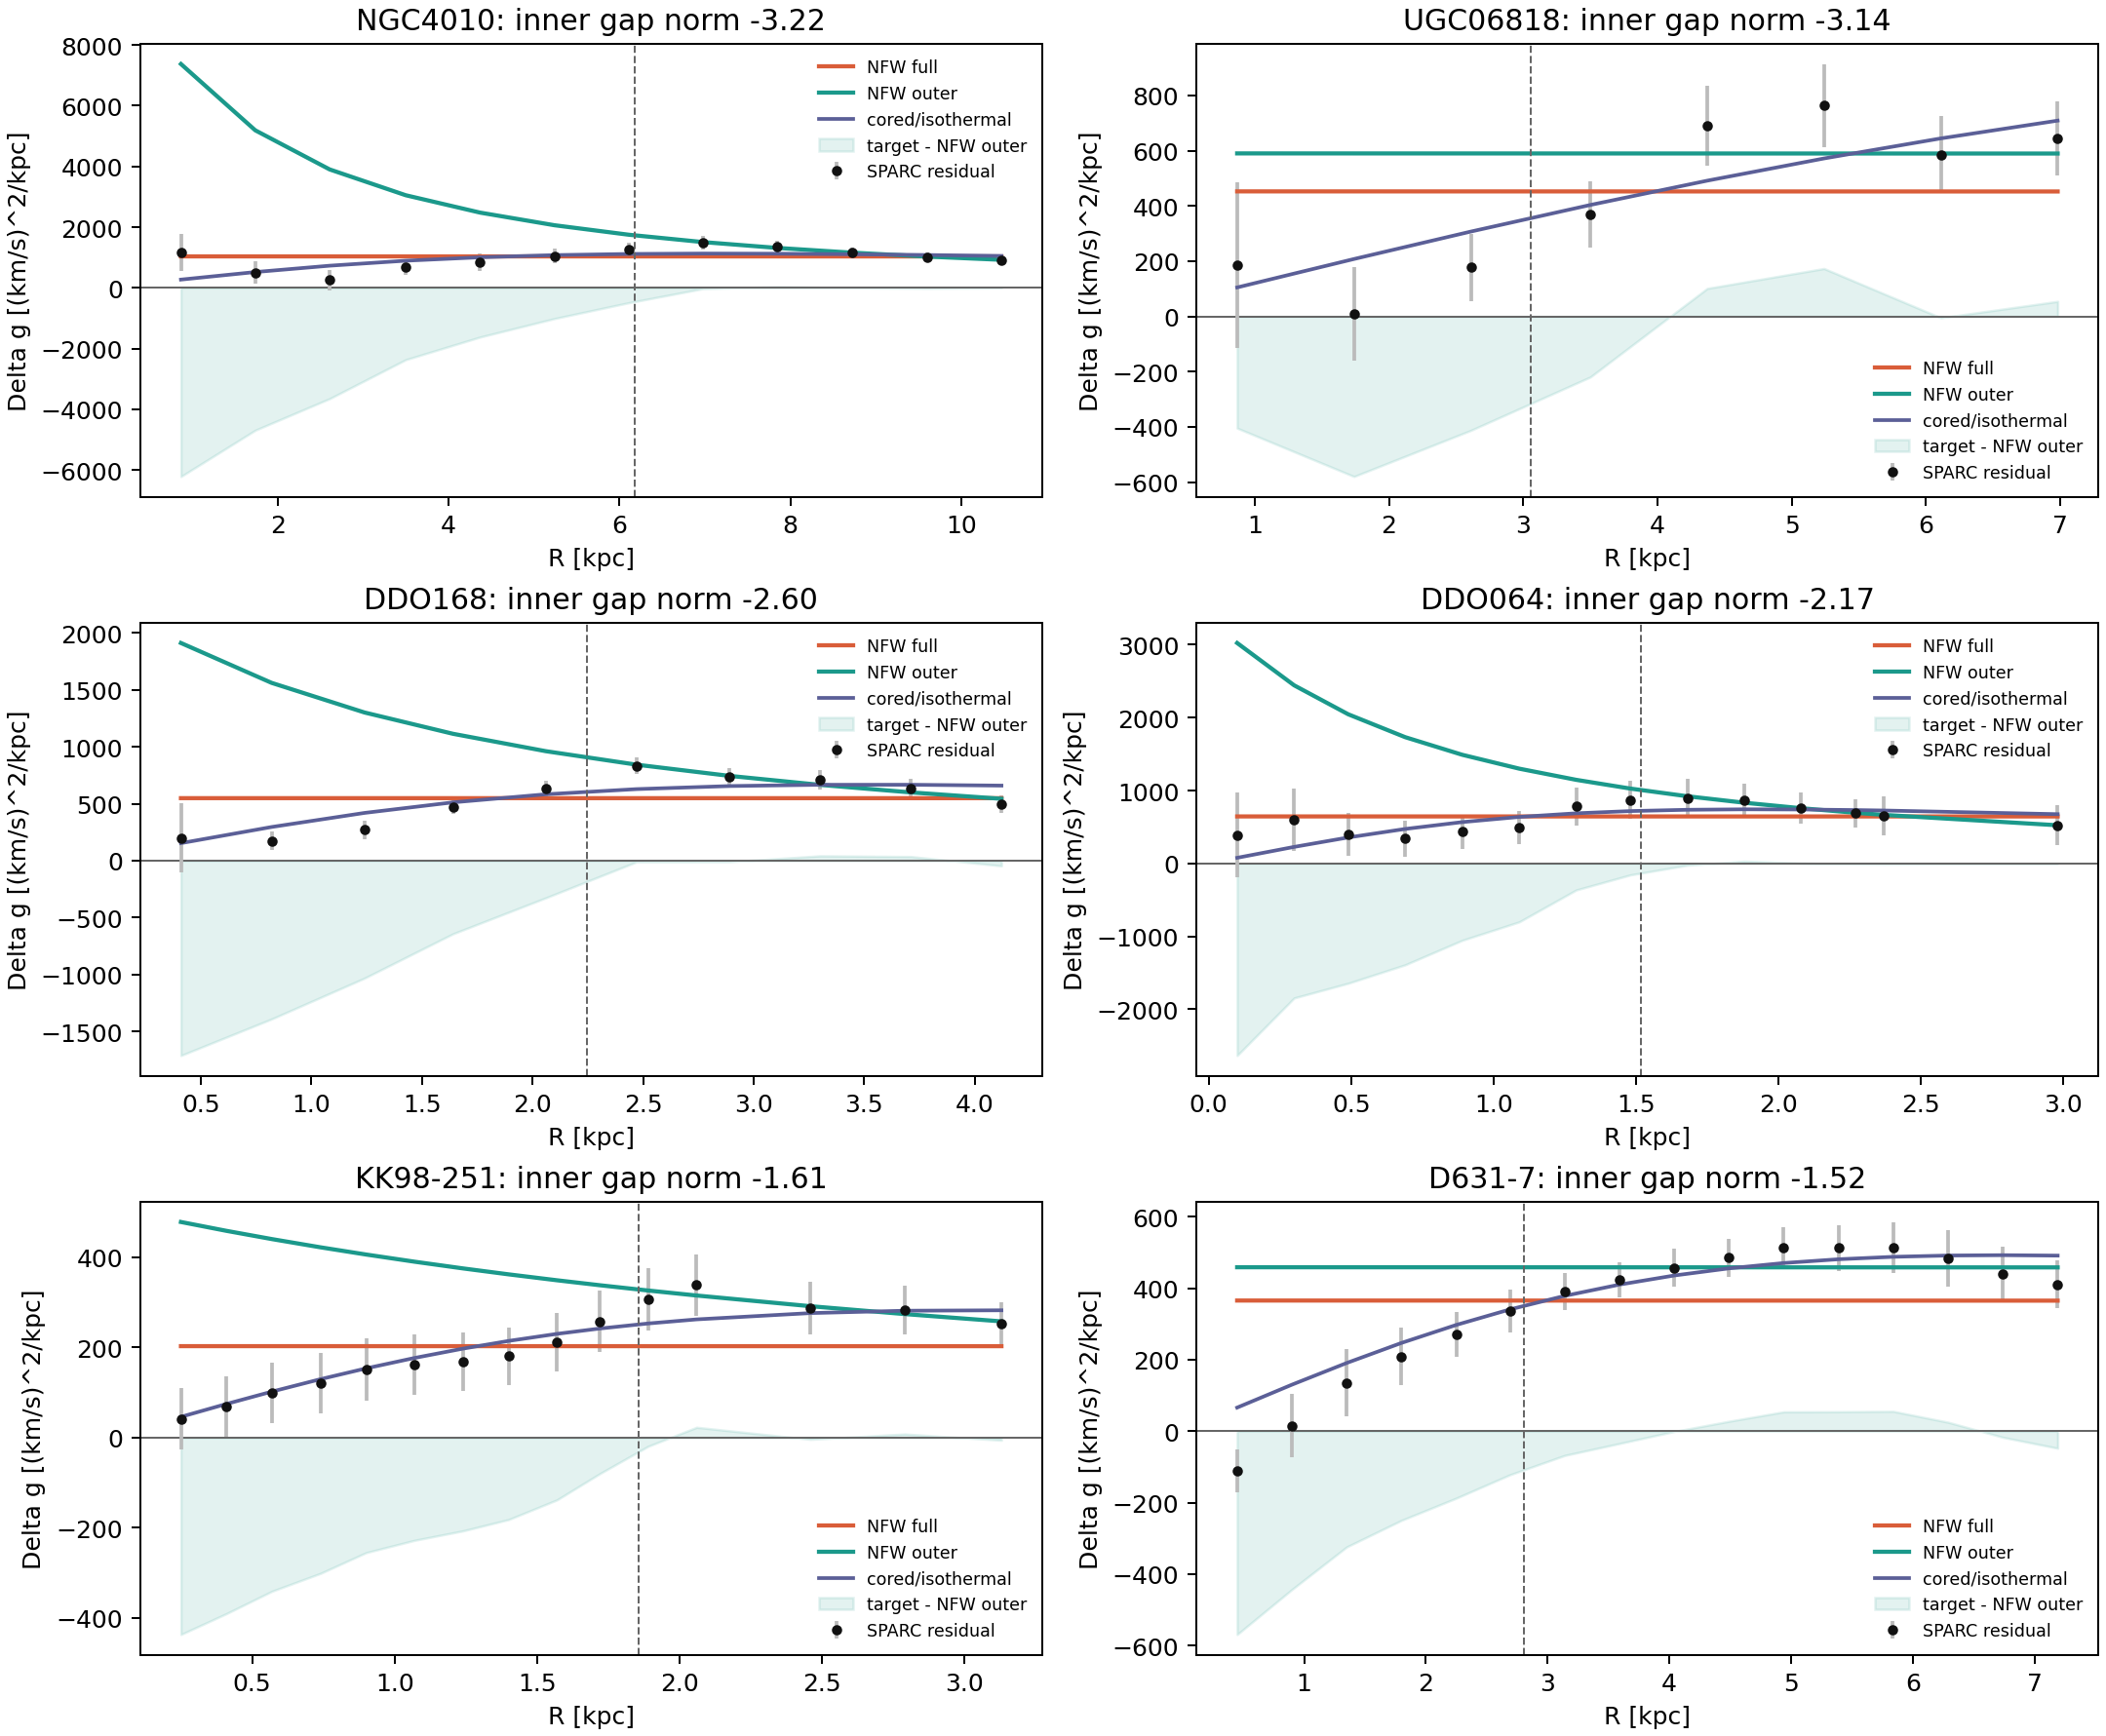
\includegraphics[width=\linewidth]{example_residual_profiles.png}
\caption{Example galaxies with strong negative inner residuals after the NFW
outer fit. The filled region is $\Delta g_{\rm obs}-\Delta g_{\rm NFW,outer}$.
The dashed vertical line marks the inner/outer split used for the outer-NFW
fit. These panels show the residual-of-residual field directly rather than only
reporting a scalar fit score.}
\label{fig:examples}
\end{figure}

\section{Results}

The first result is a direct fit comparison. In the full fitted sample,
cored/isothermal residuals beat full-range NFW fits in 78.8 percent of
galaxies. The median NFW relative RMSE is 0.337, while the median
cored/isothermal relative RMSE is 0.203. In the primary-quality sample,
cored/isothermal residuals beat NFW in 80.2 percent of galaxies, with median
relative RMSE 0.206 versus 0.334 for NFW.

The second result is the residual-of-residual diagnostic. When NFW is fit to
the outer region and then evaluated in the inner region, the primary-quality
sample has a median normalized inner gap of $-0.469$. Under the current
classification rule, 51.9 percent of primary-quality galaxies show central
overshoot: the outer-matched NFW halo leaves a structured negative inner
$\epsilon_g$. In the primary-flat subset, the overshoot fraction is 50.4
percent.

The third result is the outer-slope behavior. Full-range NFW fits often reduce
central overshoot by choosing a shape that is too shallow in the outer region.
The present diagnostic labels 74.8 percent of primary-quality full-range NFW
fits as shallow in the outer region. This is the real-data counterpart of the
synthetic result: NFW can mimic the flat-curve residual over a scale-radius
band, but fitting both the inner transition and outer tail with one pure NFW
shape is frequently difficult.

\section{Relation to Existing SPARC Halo Fits}

This result is consistent with the broader SPARC halo-fit literature. Li et al.
\citep{Li2020} fit all 175 SPARC galaxies with several dark-matter halo
families, including pISO, Burkert, NFW, Einasto, DC14, coreNFW, and Lucky13.
They report that cored halo models such as DC14 and Burkert generally fit the
rotation curves better than cuspy NFW. The present work is not a replacement
for that Bayesian halo catalog. It is a different projection of the same
problem: instead of only ranking halo profiles, it explicitly records the
leftover acceleration field $\epsilon_g(R)$ and asks whether the leftover has a
repeatable geometry.

The answer is yes. The leftover is not merely a larger chi-square. In many
galaxies it is a coherent inner negative residual when NFW is forced to match
the outer region. This converts a familiar core/cusp tension
\citep{deBlok2010} into an object that can be classified across galaxies.

\section{Limitations}

Several caveats are important. The stellar mass-to-light ratios are fixed, not
marginalized. Distance and inclination uncertainties are not varied. No
cosmological mass-concentration prior is imposed. The NFW fit is a simple
two-parameter residual fit, not a full $\Lambda$CDM halo inference. The
cored/isothermal profile is a control shape, not a claimed fundamental theory.
The density proxy is spherical and diagnostic, while SPARC galaxies are disks.
The lensing-sensitive metric potential $\Phi+\Psi$ is not constrained by these
rotation data.

Therefore the claim is methodological and empirical, not a final physical
verdict. The result does not falsify cold dark matter. It shows that
residual-of-residual geometry can be measured on public data and that simple
NFW residuals leave structured, classifiable leftover fields in a large
fraction of SPARC galaxies.

\section{Conclusion}

The synthetic NFW note \citep{Landers2026b} predicted a clear failure mode:
pure NFW can match an outer flat-curve residual or reduce central overshoot,
but it does not naturally do both in a toy target. The SPARC experiment finds
the same pattern in real data as a population tendency. Cored/isothermal
residuals beat full-range NFW fits for about 80 percent of the primary-quality
sample, and outer-NFW fits leave a structured negative inner residual in about
half of the sample.

The main contribution is the object
\begin{equation}
\boxed{
\epsilon_g(R)
=
\Delta g_{\rm obs}(R)
-
\Delta g_{\rm candidate}(R).
}
\end{equation}
It turns model mismatch into a geometric field. Once that field is measured
galaxy by galaxy, the next question is no longer just which named halo profile
has the lowest fit score. The sharper question is what physical mechanisms
produce the observed families of leftover residual geometry.

\clearpage

\begingroup\small
\begin{thebibliography}{9}

\bibitem[Landers(2026a)]{Landers2026a}
Landers, J. R. (2026a).
Geometric residuals and weak-field warp search in the missing-mass problem.
Unpublished manuscript, May 2026.

\bibitem[Landers(2026b)]{Landers2026b}
Landers, J. R. (2026b).
A residual-of-residual test of NFW geometry in the missing-mass problem.
Unpublished manuscript, May 2026.

\bibitem[Navarro et~al.(1996)]{Navarro1996}
Navarro, J. F., Frenk, C. S., \& White, S. D. M. (1996).
The structure of cold dark matter halos.
\emph{The Astrophysical Journal}, 462, 563--575.
\href{https://doi.org/10.1086/177173}{doi:10.1086/177173}.

\bibitem[Lelli et~al.(2016)]{Lelli2016}
Lelli, F., McGaugh, S. S., \& Schombert, J. M. (2016).
SPARC: Mass models for 175 disk galaxies with Spitzer photometry and accurate
rotation curves.
\emph{The Astronomical Journal}, 152, 157.
\href{https://doi.org/10.3847/0004-6256/152/6/157}{doi:10.3847/0004-6256/152/6/157}.

\bibitem[Li et~al.(2020)]{Li2020}
Li, P., Lelli, F., McGaugh, S. S., \& Schombert, J. M. (2020).
A comprehensive catalog of dark matter halo models for SPARC galaxies.
\emph{The Astrophysical Journal Supplement Series}, 247, 31.
\href{https://doi.org/10.3847/1538-4365/ab700e}{doi:10.3847/1538-4365/ab700e}.

\bibitem[McGaugh et~al.(2016)]{McGaugh2016}
McGaugh, S. S., Lelli, F., \& Schombert, J. M. (2016).
The radial acceleration relation in rotationally supported galaxies.
\emph{Physical Review Letters}, 117, 201101.
\href{https://doi.org/10.1103/PhysRevLett.117.201101}{doi:10.1103/PhysRevLett.117.201101}.

\bibitem[de Blok(2010)]{deBlok2010}
de Blok, W. J. G. (2010).
The core-cusp problem.
\emph{Advances in Astronomy}, 2010, 789293.
\href{https://doi.org/10.1155/2010/789293}{doi:10.1155/2010/789293}.

\bibitem[Bertone \& Hooper(2018)]{Bertone2018}
Bertone, G., \& Hooper, D. (2018).
History of dark matter.
\emph{Reviews of Modern Physics}, 90, 045002.
\href{https://doi.org/10.1103/RevModPhys.90.045002}{doi:10.1103/RevModPhys.90.045002}.

\end{thebibliography}
\endgroup

\end{document}
